\documentclass{ctexart}
\usepackage[hmargin=1.1in,vmargin=1in]{geometry}
\usepackage{amsmath}
\usepackage{graphicx}
\usepackage[defaultmono]{droidsansmono}

\title{《信号处理导论》课程报告四}
\input{personal_info/info.tex}

\begin{document}
    \maketitle
    \section{我学到了哪个知识点?}

    信号的正交分解。设有 $n$ 个正交函数 $\varphi_1(t), \varphi_2(t), \ldots, \varphi_n(t)$ 组成一个正交函数
    空间,用这些函数来在某一区间 $(t_1, t_2)$ 近似任一个函数 $f(t)$,即找到一组数 $C_1, C_2, \ldots, C_n$,使得
    
    \[f(t) \approx \sum_{i=1}^{n} C_i\varphi_i(t)\]

    并使得均方差
    
    \[\overline{\varepsilon^2} = \frac{1}{t_2 - t_1}\int_{t_1}^{t_2} \left[f(t) - \sum_{i=1}^{n} C_i\varphi_i(t)\right]^2\]

    最小。如果能使得 $\overline{\varepsilon^2} = 0$,则可称 $C_1\varphi_1(t), C_2\varphi_2(t), \ldots$
    是函数 $f(t)$ 在区间 $(t_1, t_2)$ 上的一个正交分解。

    \section{我之前是怎么想的?}

    我之前只在物理课和数学课上学过``矢量的正交分解'',或者说``二维向量的正交分解'',并且在线性代数课上学到过 $n$ 维
    空间的基底(一组正交的向量,且这一组向量的数量也恰好为 $n$),知道``任何一个空间向量都能被其空间的一组基底线性表示'',
    但并没想过这种概念能被推广到函数(信号)上。

    \section{我之前的想法怎么样?}

    没有推广``正交''``基底''等向量概念到信号域上。``正交分解''是后面傅里叶变换的基础,而傅里叶变换又是时域与频域相互
    转换的基础。

    \section{我应该怎样想才对?}

    信号的正交分解是在信号域上对向量的正交分解的一次推广。这种推广允许我们用一组已知正交信号线性表示任一个信号,也为后
    来的一些操作提供了方便。但是需要注意的是,这种推广并没有``100\%''保持原有的定义不变。比如说,线性代数中,$n$ 维
    向量空间的任一组基底一定包含恰好 $n$ 个向量,但是在信号域上,信号并没有``维度''的说法,并且一组``基底''也往往包
    含无穷多个信号;线性代数中的正交分解不存在误差,但是信号域上的正交分解存在误差,只是随着正交信号空间大小 $n$ 趋近
    于 0,误差也趋近于 0,所以才可以将一个信号 $f(t)$ 正交分解为一个无穷级数 $\sum_{i=1}^{n} C_i\varphi_i(t)$。

    \section{我应该怎样用上它?}

    信号的正交分解是对已有概念的一次推广,将其他学科的内容推广至本学科,从而得到一些重要的工具来解决本学科的问题。在日常
    生活与学习中我们也应当注意多加尝试推广已知,尝试利用已知的内容来构造出未解决问题的解,从而解决问题。但是还需注意的
    是,推广不是生搬硬套,比如信号正交分解在推广向量正交分解的过程中就引入了``均方差'',并修改了其他部分概念的定义,从
    而使得``解''更加符合实际需求。

    \section*{字数统计}

    \begin{center}
        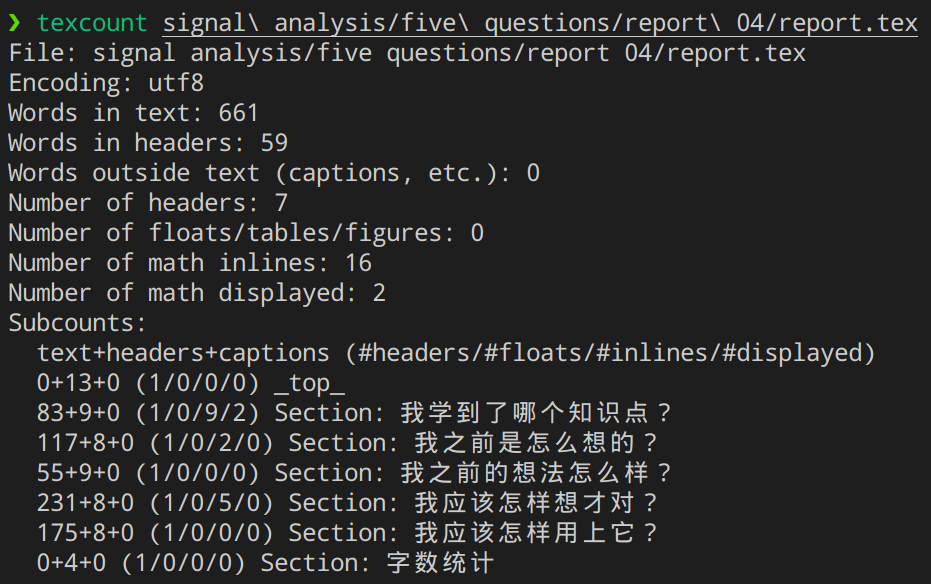
\includegraphics[width=0.7\textwidth]{pics/texcount.png}
    \end{center}
\end{document}